\documentclass[12pt]{article}
\usepackage[margin=2.5cm]{geometry}
\usepackage{enumerate}
\usepackage{amsfonts}
\usepackage{amsmath}
\usepackage{fancyhdr}
\usepackage{amsmath}
\usepackage{amssymb}
\usepackage{amsthm}
\usepackage{mdframed}
\usepackage{graphicx}
\usepackage{subcaption}
\usepackage{adjustbox}
\usepackage{listings}
\usepackage{xcolor}
\usepackage{booktabs}
\usepackage[utf]{kotex}
\usepackage{hyperref}

\definecolor{codegreen}{rgb}{0,0.6,0}
\definecolor{codegray}{rgb}{0.5,0.5,0.5}
\definecolor{codepurple}{rgb}{0.58,0,0.82}
\definecolor{backcolour}{rgb}{0.95,0.95,0.92}

\lstdefinestyle{mystyle}{
    backgroundcolor=\color{backcolour},
    commentstyle=\color{codegreen},
    keywordstyle=\color{magenta},
    numberstyle=\tiny\color{codegray},
    stringstyle=\color{codepurple},
    basicstyle=\ttfamily\footnotesize,
    breakatwhitespace=false,
    breaklines=true,
    captionpos=b,
    keepspaces=true,
    numbers=left,
    numbersep=5pt,
    showspaces=false,
    showstringspaces=false,
    showtabs=false,
    tabsize=1
}

\lstset{style=mystyle}

\pagestyle{fancy}
\renewcommand{\headrulewidth}{0.4pt}
\lhead{CSC 369}
\rhead{Worksheet 5 Solution}

\begin{document}
\title{CSC 369 Worksheet 5 Solution}
\maketitle

\bigskip

\begin{enumerate}[1.]
    \item

    \bigskip

    I need to run randomly-generated problems with two jobs and two queues using
    file \texttt{mlfq.py} with I/O turned off, and compute the MLFQ execution trace for each.

    \bigskip

    Using the command \texttt{./mlfq.py -s 1 -m 10 -n 2 -j 2 -M 0}, we have

    \bigskip

    \begin{center}
    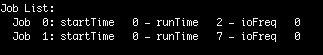
\includegraphics[width=0.6\linewidth]{images/worksheet_5_solution_3.png}
    \end{center}

    with

    \begin{itemize}
        \item allotments for queue 1 is 1
        \item quantum length for queue 1 is 10
        \item allotments for queue 0 is 1
        \item quantum length for queue 0 is 10
        \item no priority boost
    \end{itemize},

    the exeuction trace is:

    \bigskip

\begin{lstlisting}
    [time 0] Job begins by job 0
    [time 0] Job begins by job 1
    [time 0] Run job 0 at priority 1 [Ticks 9, Allotment 1, Time 1 (of 2)]
    [time 1] Run job 0 at priority 1 [Ticks 8, Allotment 1, Time 0 (of 2)]
    [time 2] Finished JOB 0
    [time 2] Run job 1 at priority 1 [Ticks 9, Allotment 1, Time 6 (of 7)]
    [time 3] Run job 1 at priority 1 [Ticks 8, Allotment 1, Time 5 (of 7)]
    [time 4] Run job 1 at priority 1 [Ticks 7, Allotment 1, Time 4 (of 7)]
    [time 5] Run job 1 at priority 1 [Ticks 6, Allotment 1, Time 3 (of 7)]
    [time 6] Run job 1 at priority 1 [Ticks 5, Allotment 1, Time 2 (of 7)]
    [time 7] Run job 1 at priority 1 [Ticks 4, Allotment 1, Time 1 (of 7)]
    [time 8] Run job 1 at priority 1 [Ticks 3, Allotment 1, Time 0 (of 7)]
    [time 9] Finished JOB 1
\end{lstlisting}

    \bigskip

    \underline{\textbf{Notes}}

    \begin{itemize}
        \item Learned that when alloted time is up, the next job starts immediately

        \begin{center}
        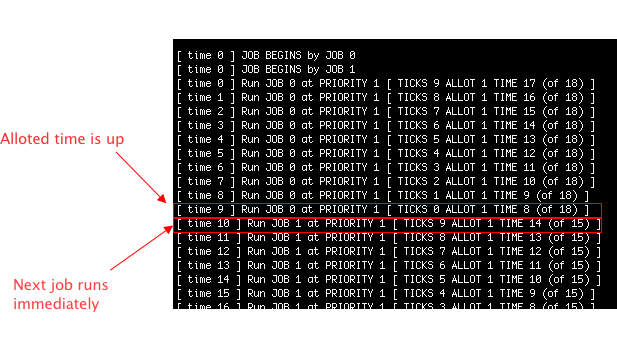
\includegraphics[width=0.9\linewidth]{images/worksheet_5_solution_4.png}
        \end{center}

        \item Learned that when all jobs are at the bottom, without priority boost, jobs finishes by round robin
        \item Learned that notification and subsequent job execution happen at the same time.
        \item The reason why round robin doesn't occur despite $\text{Priority(A)} = \text{Priority(B)}$
        is because allotment of queue is 1 (i.e. only one job can be in a queue)
        \item \textbf{allotment} means the amount of something allocated to a person/object (i.e. the size of queue)
        \item \texttt{-m 10} sets the maximum runtime of a job to 10
        \item \texttt{-M 0} turns off I/O in \texttt{mlfq.py}
        \item \texttt{-n 2} sets number of queues to 2
        \item \texttt{-j 2} sets number of jobs to 2

        \item \textbf{Multi-level Feeback Queue (MLFQ):}

        \begin{itemize}
            \item Is one of the most well-known approaches to scheduling
            \item Does two things:

            \begin{enumerate}[a)]
                \item Optimizes turnaround time
                \item Minimizes response time
            \end{enumerate}

            \item Uses \textbf{priority level} and \textbf{Queues} to achieve it's goal
        \end{itemize}

        \item \textbf{MLFQ Basic Rules:}
        \begin{itemize}
            \item Jobs on same queue $\to$ Same priority
            \item \textbf{Rule 1:} If $\text{Priority(A)} > \text{Priority(B)}$, A runs (B doesn't)
            \item \textbf{Rule 2:} If $\text{Priority(A)} = \text{Priority(B)}$, A \& B run in RR
        \end{itemize}

        \bigskip

        \begin{center}
        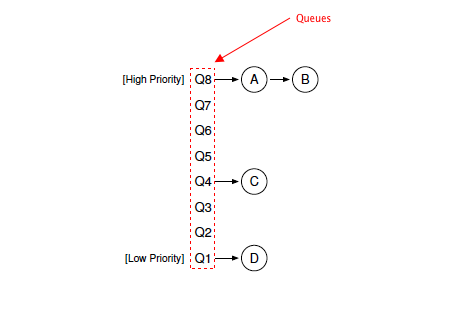
\includegraphics[width=0.8\linewidth]{images/worksheet_5_solution_1.png}
        \end{center}

        \item \textbf{Attemp \#1: How to Change Priority}

        \begin{itemize}
            \item \textbf{Rule 3:} When a job enters the system, it is placed at the \underline{highest}
            priority (the topmost queue)
            \item \textbf{Rule 4a:} If a job uses up an entire time slice while running , its' priority is
            \underline{reduced} (i.e. it moves down on queue).
            \item \textbf{Rule 4b:} If a job gives up the CPU before the time slice is up, it stays
            at the \underline{same} priority level (e.g I/O Operation)

            \begin{itemize}
                \item Means that the shifting down of priority level only depends on CPU time
            \end{itemize}

            \bigskip

            \underline{\textbf{Example (Along Came a Short Job):}}

            \bigskip

            \begin{enumerate}[1)]
                \item A job $A$ enters system
                \item Job is placed on highest Queue $Q_2$
                \item After time-slice (e.g. 10 ms) in $Q_2$, $A$ is placed on lower queue $Q_1$
                \item After time-slice in $Q_1$, $A$ is placed in lowest priority queue $Q_0$
            \end{enumerate}

            \begin{center}
            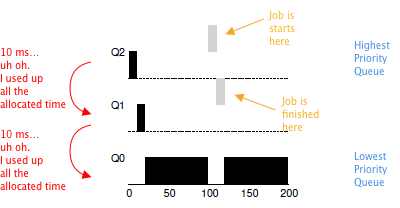
\includegraphics[width=0.8\linewidth]{images/worksheet_5_solution_2.png}
            \end{center}
        \end{itemize}

        \item \textbf{Attemp \#2: The Priority Boost}

        \begin{itemize}
            \item \textbf{Rule 5:} After some time period $S$, move all the jobs in the system
            to the topmost queue.

            \begin{itemize}
                \item This is to prevent starvation (i.e. a job never being run)
            \end{itemize}
        \end{itemize}

        \item \textbf{Attempt \#3: Better Accounting (Fix of Attempt \# 1)}

        \begin{itemize}
            \item Is to prevent programmers from gaming (i.e tricking) the CPU so
            all programs get a fair share of allotment time
            \item \textbf{Rule 4:} Once a job uses up its time allotment at a given level
            (regardless of how many times it has given up the CPU), its priority is reduced
            (it moves down one queue).
        \end{itemize}


    \end{itemize}
\end{enumerate}

\end{document}